% Options for packages loaded elsewhere
\PassOptionsToPackage{unicode}{hyperref}
\PassOptionsToPackage{hyphens}{url}
\PassOptionsToPackage{dvipsnames,svgnames,x11names}{xcolor}
%
\documentclass[
  10pt,
  letterpaper,
  oneside,
  open=any]{scrbook}

\usepackage{amsmath,amssymb}
\usepackage{iftex}
\ifPDFTeX
  \usepackage[T1]{fontenc}
  \usepackage[utf8]{inputenc}
  \usepackage{textcomp} % provide euro and other symbols
\else % if luatex or xetex
  \usepackage{unicode-math}
  \defaultfontfeatures{Scale=MatchLowercase}
  \defaultfontfeatures[\rmfamily]{Ligatures=TeX,Scale=1}
\fi
\usepackage{lmodern}
\ifPDFTeX\else  
    % xetex/luatex font selection
  \setmainfont[]{Georgia}
  \setsansfont[]{Verdana}
\fi
% Use upquote if available, for straight quotes in verbatim environments
\IfFileExists{upquote.sty}{\usepackage{upquote}}{}
\IfFileExists{microtype.sty}{% use microtype if available
  \usepackage[final]{microtype}
  \UseMicrotypeSet[protrusion]{basicmath} % disable protrusion for tt fonts
}{}
\makeatletter
\@ifundefined{KOMAClassName}{% if non-KOMA class
  \IfFileExists{parskip.sty}{%
    \usepackage{parskip}
  }{% else
    \setlength{\parindent}{0pt}
    \setlength{\parskip}{6pt plus 2pt minus 1pt}}
}{% if KOMA class
  \KOMAoptions{parskip=half}}
\makeatother
\usepackage{xcolor}
\usepackage[margin=0.5in,bindingoffset=0.0in]{geometry}
\setlength{\emergencystretch}{3em} % prevent overfull lines
\setcounter{secnumdepth}{5}
% Make \paragraph and \subparagraph free-standing
\ifx\paragraph\undefined\else
  \let\oldparagraph\paragraph
  \renewcommand{\paragraph}[1]{\oldparagraph{#1}\mbox{}}
\fi
\ifx\subparagraph\undefined\else
  \let\oldsubparagraph\subparagraph
  \renewcommand{\subparagraph}[1]{\oldsubparagraph{#1}\mbox{}}
\fi


\providecommand{\tightlist}{%
  \setlength{\itemsep}{0pt}\setlength{\parskip}{0pt}}\usepackage{longtable,booktabs,array}
\usepackage{calc} % for calculating minipage widths
% Correct order of tables after \paragraph or \subparagraph
\usepackage{etoolbox}
\makeatletter
\patchcmd\longtable{\par}{\if@noskipsec\mbox{}\fi\par}{}{}
\makeatother
% Allow footnotes in longtable head/foot
\IfFileExists{footnotehyper.sty}{\usepackage{footnotehyper}}{\usepackage{footnote}}
\makesavenoteenv{longtable}
\usepackage{graphicx}
\makeatletter
\def\maxwidth{\ifdim\Gin@nat@width>\linewidth\linewidth\else\Gin@nat@width\fi}
\def\maxheight{\ifdim\Gin@nat@height>\textheight\textheight\else\Gin@nat@height\fi}
\makeatother
% Scale images if necessary, so that they will not overflow the page
% margins by default, and it is still possible to overwrite the defaults
% using explicit options in \includegraphics[width, height, ...]{}
\setkeys{Gin}{width=\maxwidth,height=\maxheight,keepaspectratio}
% Set default figure placement to htbp
\makeatletter
\def\fps@figure{htbp}
\makeatother

\usepackage{booktabs}
\usepackage{longtable}
\usepackage{array}
\usepackage{multirow}
\usepackage{wrapfig}
\usepackage{float}
\usepackage{colortbl}
\usepackage{pdflscape}
\usepackage{tabu}
\usepackage{threeparttable}
\usepackage{threeparttablex}
\usepackage[normalem]{ulem}
\usepackage{makecell}
\usepackage{xcolor}
\usepackage{amssymb}
\usepackage{pifont}
\usepackage{wasysym}
\titlehead{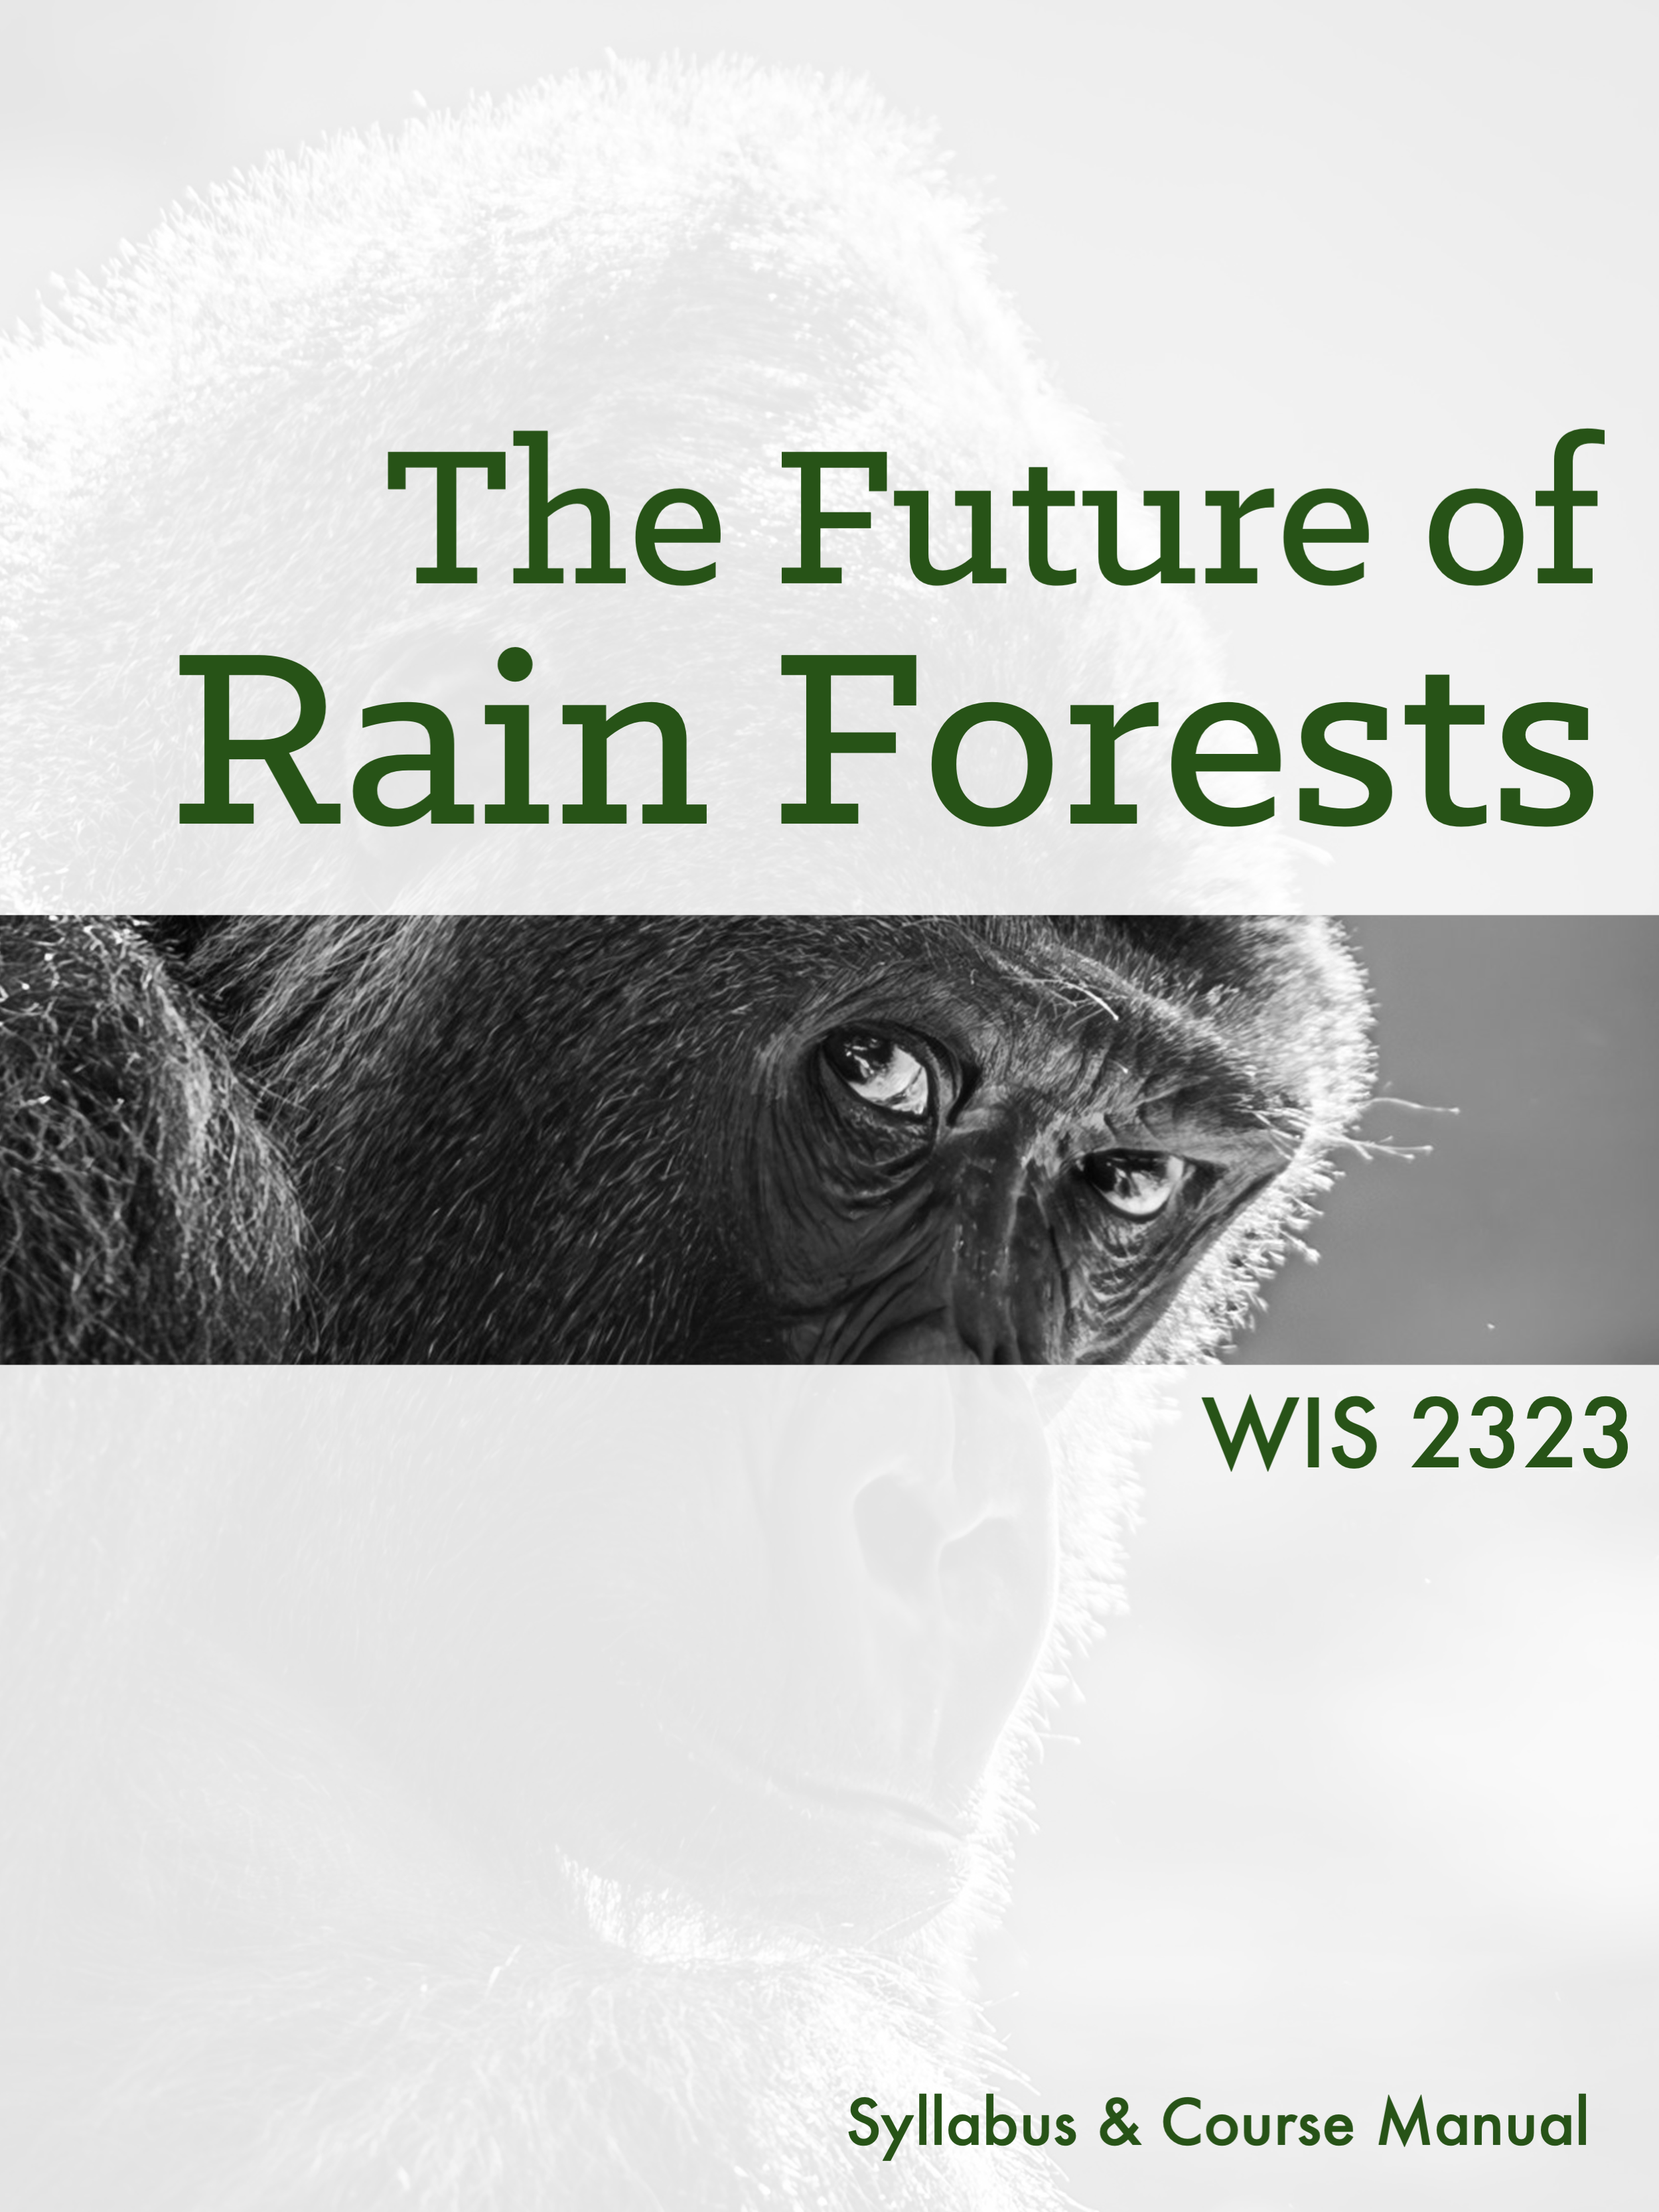
\includegraphics[height=9in]{images/cover.png}}
\publishers{v0.9.0 (Zenodo https://doi.org/10.5281/zenodo.14232308)\\-\\This material is based upon work supported by the National Science Foundation under Award No. NSF DEB-2203582.\\-\\Licensed under CC BY-NC-SA 4.0.}
\makeatletter
\@ifpackageloaded{tcolorbox}{}{\usepackage[skins,breakable]{tcolorbox}}
\@ifpackageloaded{fontawesome5}{}{\usepackage{fontawesome5}}
\definecolor{quarto-callout-color}{HTML}{909090}
\definecolor{quarto-callout-note-color}{HTML}{0758E5}
\definecolor{quarto-callout-important-color}{HTML}{CC1914}
\definecolor{quarto-callout-warning-color}{HTML}{EB9113}
\definecolor{quarto-callout-tip-color}{HTML}{00A047}
\definecolor{quarto-callout-caution-color}{HTML}{FC5300}
\definecolor{quarto-callout-color-frame}{HTML}{acacac}
\definecolor{quarto-callout-note-color-frame}{HTML}{4582ec}
\definecolor{quarto-callout-important-color-frame}{HTML}{d9534f}
\definecolor{quarto-callout-warning-color-frame}{HTML}{f0ad4e}
\definecolor{quarto-callout-tip-color-frame}{HTML}{02b875}
\definecolor{quarto-callout-caution-color-frame}{HTML}{fd7e14}
\makeatother
\makeatletter
\@ifpackageloaded{bookmark}{}{\usepackage{bookmark}}
\makeatother
\makeatletter
\@ifpackageloaded{caption}{}{\usepackage{caption}}
\AtBeginDocument{%
\ifdefined\contentsname
  \renewcommand*\contentsname{Table of contents}
\else
  \newcommand\contentsname{Table of contents}
\fi
\ifdefined\listfigurename
  \renewcommand*\listfigurename{List of Figures}
\else
  \newcommand\listfigurename{List of Figures}
\fi
\ifdefined\listtablename
  \renewcommand*\listtablename{List of Tables}
\else
  \newcommand\listtablename{List of Tables}
\fi
\ifdefined\figurename
  \renewcommand*\figurename{Figure}
\else
  \newcommand\figurename{Figure}
\fi
\ifdefined\tablename
  \renewcommand*\tablename{Table}
\else
  \newcommand\tablename{Table}
\fi
}
\@ifpackageloaded{float}{}{\usepackage{float}}
\floatstyle{ruled}
\@ifundefined{c@chapter}{\newfloat{codelisting}{h}{lop}}{\newfloat{codelisting}{h}{lop}[chapter]}
\floatname{codelisting}{Listing}
\newcommand*\listoflistings{\listof{codelisting}{List of Listings}}
\makeatother
\makeatletter
\makeatother
\makeatletter
\@ifpackageloaded{caption}{}{\usepackage{caption}}
\@ifpackageloaded{subcaption}{}{\usepackage{subcaption}}
\makeatother
\makeatletter
\@ifpackageloaded{fontawesome5}{}{\usepackage{fontawesome5}}
\makeatother
\ifLuaTeX
  \usepackage{selnolig}  % disable illegal ligatures
\fi
\usepackage{bookmark}

\IfFileExists{xurl.sty}{\usepackage{xurl}}{} % add URL line breaks if available
\urlstyle{same} % disable monospaced font for URLs
\hypersetup{
  pdftitle={Syllabus: The Future of Rain Forests (WIS 2323)},
  colorlinks=true,
  linkcolor={Maroon},
  filecolor={Maroon},
  citecolor={Blue},
  urlcolor={Blue},
  pdfcreator={LaTeX via pandoc}}

\title{Syllabus: The Future of Rain Forests (WIS 2323)}
\author{}
\date{}

\begin{document}
\frontmatter
\maketitle

\renewcommand*\contentsname{Table of Contents}
{
\hypersetup{linkcolor=}
\setcounter{tocdepth}{0}
\tableofcontents
}
\mainmatter
\bookmarksetup{startatroot}

\chapter{Course Overview}\label{course-overview}

\subsection*{Course Description}\label{course-description}
\addcontentsline{toc}{subsection}{Course Description}

This course investigates the fundamental issues addressed by scientists
studying tropical rain forests, including what gave rise to their
remarkable biodiversity, the drivers and consequences of deforestation,
why people are fascinated by rain forests, cultural stereotypes about
the tropics, and if forest conservation is compatible with socioeconomic
development. \textbf{\emph{By the end of the course students will be
able to:}}

\begin{itemize}
\tightlist
\item
  Recognize and describe stereotypes about rain forests \& their
  residents
\item
  Analyze rain forest tropes in art, literature, \& popular culture
\item
  Discuss \& evaluate hypotheses for the origins and maintenance of
  tropical biodiversity
\item
  Explain \& compare human history in rain forests
\item
  Review contemporary threats to rain forests
\item
  Analyze and visualize data on deforestation
\item
  Review and contrast strategies for rain forest conservation \&
  restoration
\item
  Identify rain forests in their daily lives \& set personal goals for
  advancing their conservation
\item
  Produce materials for communicating about rain forests to family and
  peers
\end{itemize}

\subsection*{When \& Where}\label{when-where}
\addcontentsline{toc}{subsection}{When \& Where}

\textbf{When:} Tuesdays 3:00-3:50 and Thursdays 3:00-4:55\\
\textbf{Where:} LIT 0231 (both days)

\subsection*{Instructor \& TA}\label{instructor-ta}
\addcontentsline{toc}{subsection}{Instructor \& TA}

\textbf{Instructor:} Dr.~Emilio M. Bruna\\
email: embruna@ufl.edu\\
phone: (352) 846-0634\\
Office: Tropical Ecology \& Conservation Lab, 711 Newell Dr.

\textbf{TA:} Priyanka Hari Haran\\
email: phariharan1@ufl.edu\\
Phone: (352) 846-0527\\
Office: Tropical Ecology \& Conservation Lab, 711 Newell Dr.

\begin{center}\rule{0.5\linewidth}{0.5pt}\end{center}

\bookmarksetup{startatroot}

\chapter{GenEd, Quest, \& Credit
Information}\label{gened-quest-credit-information}

\textbf{A minimum grade of C is required for Quest and General Education
credit.} Courses intended to satisfy Quest and General Education
requirements cannot be taken S-U. \emph{This course fulfills the
following Quest and GenEd requirements:}

\begin{itemize}
\tightlist
\item
  Quest 2
\item
  GenEd International
\item
  \emph{Credits:} 3
\item
  \emph{Prerequisites:} None
\end{itemize}

\section*{Credit towards Minors \&
Certificates}\label{credit-towards-minors-certificates}
\addcontentsline{toc}{section}{Credit towards Minors \& Certificates}

\markright{Credit towards Minors \& Certificates}

\textbf{This also counts towards a minor or certificate in Latin
American Studies.}\\
See
\href{https://www.latam.ufl.edu/academics/undergraduate-programs/}{www.latam.ufl.edu/academics/undergraduate-programs}
for more information.

\bookmarksetup{startatroot}

\chapter{Required Course Materials}\label{required-course-materials}

\textbf{Students are not required to purchase any textbooks or course
materials;} all materials, including readings and videos, will be
available on the course Canvas page. However, many of the assigned
readings from the \emph{New York Times} and \emph{Washington Post} have
dynamic multimedia data visualizations and video that can't be
appreciated in the posted .pdf format. \emph{Students in this class
should sign up for free online access to the New York Times} and
\emph{Washington Post} by following the instructions at
\href{https://businesslibrary.uflib.ufl.edu/c.php?g=943928&p=7708734}{this
UF Libraries Website}.

\textbf{Materials and Supplies Fees}: None.

\bookmarksetup{startatroot}

\chapter{Office Hours}\label{office-hours}

\textbf{Instructor:} Wednesday \& Friday 1:30-3:00 pm or by appointment
(in-person \& online). Drop by anytime or sign up for a specific time
here: \url{https://embruna.youcanbook.me}.

\textbf{Teaching Assistant:} Tuesday 1:00-2:30 pm or by appointment
(in-person \& online).

\textbf{\emph{Location: In-person:}} The Tropical Ecology \&
Conservation Lab is located next to the Rawlings Hall bus stop (711
Newell Drive; to find a map click the ``Contact'' link at
\href{http://brunalab.org}{BrunaLab.org}). \textbf{\emph{Location -
online:}} use the zoom link on the course Canvas page. We are online the
entire session.

\bookmarksetup{startatroot}

\chapter{Assignments, Grades, \&
Attendance}\label{assignments-grades-attendance}

Learning in our class is achieved with an diverse array of methods
ranging from data analysis to essays to projects. In most class sessions
you will also be working with small groups of students to complete an
in-class assignment that reinforces the major themes of the day's topic.
In keeping with the philosophy of the Quest program, this course also
has \emph{Experiential Learning and Self-Reflection Components}. For
details on the different types of assignments and the Quest Learning
Components, see the course Canvas page.

\subsection{Assignments (1000 points
total)}\label{assignments-1000-points-total}

\begin{center}
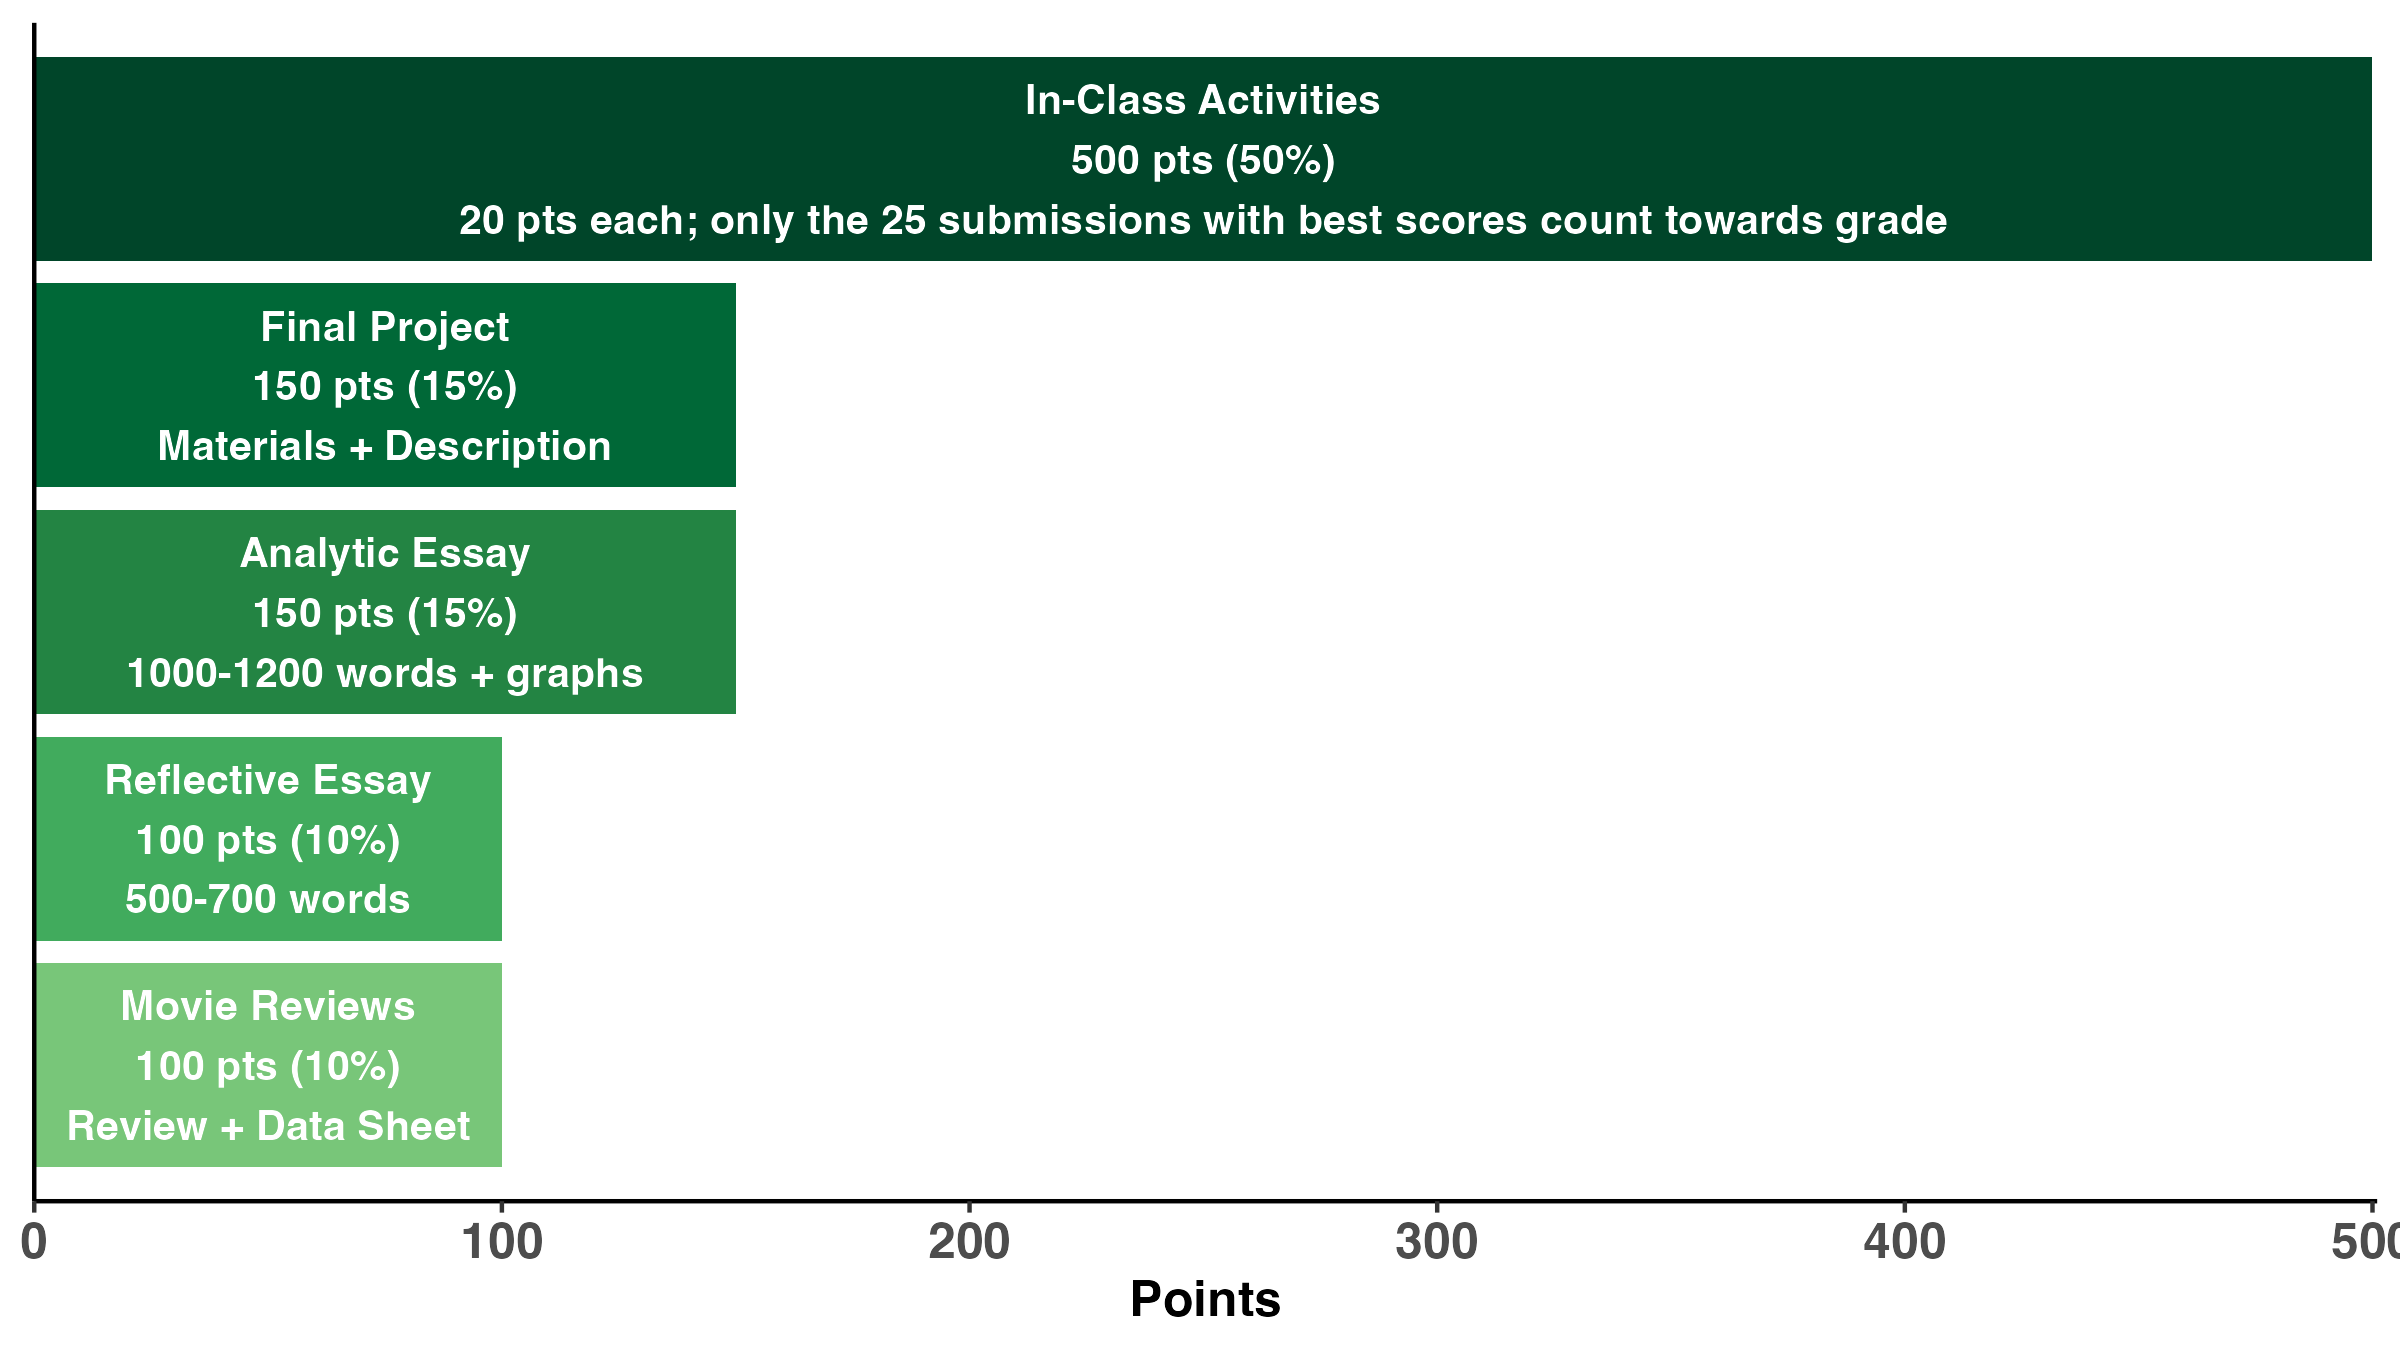
\includegraphics[width=1\textwidth,height=\textheight]{images/hw.png}
\end{center}

\subsection{Grading}\label{grading}

\textbf{In-class Assignments are due by the following class session.}
Late assignments will lose 10 pts.

\textbf{\emph{Regrades:}} Requests for re-evaluation of assignments must
be accompanied by an explanation for why you think you deserve
additional credit and the number of additional points you think you
deserve. The deadline for submission is one week after the work was
returned.

\textbf{\emph{Grade Assignment}} (based on \% of total points earned): A
= 94--100\%, A- = 90--93\%, B+ = 87--89\%, B = 84--86\%, B- = 80--83\%,
C+ = 77--79\%, C = 74--76\%, C- = 70--73\%, D+ = 67--69\%, D = 64--66\%,
D- = 60--63\%, E\textless60

\textbf{\emph{Grade Points:}} For information on how UF assigns grade
points, visit:
\url{https://catalog.ufl.edu/UGRD/academic-regulations/grades-grading-policies/}

\subsection{Attendance \& Participation}\label{attendance-participation}

\textbf{\emph{Attendance:}} Though attendance is not required, many of
the sessions we will be completing activities in class that count
towards your grade. Most of these can be completed independently, but by
doing them in class you will benefit from working collaboratively with
the other students.

\textbf{Some of the in-class activities can only be completed in that
day's class session.} If you miss class on one one of these days, that
is why the grade for in-class activities is based on a subset of the
total activities; you can also elect to make up lost points with
extra-credit assignments. \textbf{\emph{If you need to miss class for
any reason, please let me know as soon as possible}}. We will make
arrangements for you to complete any assignments and go over any
material you will be missing. I would much rather you focus on your
health, attend your conference, or support friends and family in need
than struggle to turn in assignments.

\textbf{\emph{Participation:}} Consistent informed, thoughtful, and
considerate class participation is encouraged (and in some cases
required). \emph{If you have personal issues that prohibit you from
joining freely in class discussion (e.g., shyness, language barriers,
medical condition): no problem.} let us know and we will discuss
alternative modes of participation.

\begin{tcolorbox}[enhanced jigsaw, toptitle=1mm, arc=.35mm, opacitybacktitle=0.6, colbacktitle=quarto-callout-tip-color!10!white, titlerule=0mm, colback=white, opacityback=0, colframe=quarto-callout-tip-color-frame, coltitle=black, left=2mm, toprule=.15mm, title=\textcolor{quarto-callout-tip-color}{\faLightbulb}\hspace{0.5em}{Important note regarding class discussions and group work.}, breakable, leftrule=.75mm, bottomtitle=1mm, rightrule=.15mm, bottomrule=.15mm]

We will explore some challenging, important problems and increase our
understandings of different perspectives and approaches for addressing
them. These conversations may not always be easy; we sometimes will make
mistakes in both how we communicate our perspective and what we hear
other say. There may be times when we need patience, courage,
imagination, and of course mutual respect to engage our texts,
classmates, instructors, guests, and our own ideas and experiences.
\emph{Disrespectful or disruptive behavior will not be tolerated}. And
always remember that as scholars we must employ critical thinking, rely
on data, and cite verifiable sources and experts to interrogate all
assigned readings and subject matter in this course as a means of
determining if we agree with classmates and instructors. No lesson is
intended to espouse, promote, advance, inculcate, or compel a particular
feeling, perception, viewpoint or belief.

\end{tcolorbox}

\bookmarksetup{startatroot}

\chapter{Semester Calendar \& Key
Dates}\label{semester-calendar-key-dates}

\begingroup\fontsize{9}{11}\selectfont

\begin{longtable*}[l]{>{\centering\arraybackslash}p{7em}>{\centering\arraybackslash}p{1em}>{\centering\arraybackslash}p{8em}>{\raggedright\arraybackslash}p{25em}>{}r}
\toprule
\cellcolor[HTML]{1F691B}{\textcolor{white}{\textbf{\textbf{WEEK}}}} & \cellcolor[HTML]{1F691B}{\textcolor{white}{\textbf{\textbf{}}}} & \cellcolor[HTML]{1F691B}{\textcolor{white}{\textbf{\textbf{DATE}}}} & \cellcolor[HTML]{1F691B}{\textcolor{white}{\textbf{\textbf{TOPIC}}}} & \cellcolor[HTML]{1F691B}{\textcolor{white}{\textbf{\textbf{ASSIGNMENT INFO}}}}\\
\midrule
\addlinespace[0.3em]
\multicolumn{5}{l}{\textbf{WHY ARE WE FASCINATED BY TROPICAL RAIN FORESTS?}}\\
\hspace{1em}Week 1 & \cellcolor{white}{1} & 22-Aug & Class Starts Thursday! & \textbf{}\\
\hspace{1em} & \cellcolor{white}{2} & 21-Aug & Course Welcome and Introduction & \textbf{}\\
\cellcolor[HTML]{D3D3D3}{\hspace{1em}} & \cellcolor[HTML]{D3D3D3}{} & \cellcolor[HTML]{D3D3D3}{} & \cellcolor[HTML]{D3D3D3}{ \vphantom{15}} & \cellcolor[HTML]{D3D3D3}{\textbf{}}\\
\hspace{1em}Week 2 & \cellcolor{white}{1} & 26-Aug & Historical Narratives & \textbf{}\\
\hspace{1em} & \cellcolor{white}{2} & 28-Aug & Rain forest imagery in Art \& Lit & \textbf{}\\
\cellcolor[HTML]{D3D3D3}{\hspace{1em}} & \cellcolor[HTML]{D3D3D3}{} & \cellcolor[HTML]{D3D3D3}{} & \cellcolor[HTML]{D3D3D3}{ \vphantom{14}} & \cellcolor[HTML]{D3D3D3}{\textbf{}}\\
\hspace{1em}Week 3 & \cellcolor{white}{1} & 2-Sep & The Rain Forest in Pop Culture & \textbf{Movie Reviews Assigned}\\
\addlinespace[0.3em]
\multicolumn{5}{l}{\textbf{THE ECOLOGY \& EVOLUTION OF TROPICAL RAIN FORESTS}}\\
\hspace{1em} & \cellcolor{white}{2} & 4-Sep & What is a Rain Forest? & \textbf{}\\
\cellcolor[HTML]{D3D3D3}{\hspace{1em}} & \cellcolor[HTML]{D3D3D3}{} & \cellcolor[HTML]{D3D3D3}{} & \cellcolor[HTML]{D3D3D3}{ \vphantom{13}} & \cellcolor[HTML]{D3D3D3}{\textbf{}}\\
\hspace{1em}Week 4 & \cellcolor{white}{1} & 9-Sep & What else is a Rain Forest? & \textbf{}\\
\hspace{1em} & \cellcolor{white}{2} & 11-Sep & Patterns of Biodiversity 1 & \textbf{}\\
\cellcolor[HTML]{D3D3D3}{\hspace{1em}} & \cellcolor[HTML]{D3D3D3}{} & \cellcolor[HTML]{D3D3D3}{} & \cellcolor[HTML]{D3D3D3}{ \vphantom{12}} & \cellcolor[HTML]{D3D3D3}{\textbf{}}\\
\hspace{1em}Week 5 & \cellcolor{white}{1} & 16-Sep & Patterns of Biodiversity 2 & \textbf{}\\
\hspace{1em} & \cellcolor{white}{2} & 18-Sep & Origins of tropical biodiversity & \textbf{}\\
\cellcolor[HTML]{D3D3D3}{\hspace{1em}} & \cellcolor[HTML]{D3D3D3}{} & \cellcolor[HTML]{D3D3D3}{} & \cellcolor[HTML]{D3D3D3}{ \vphantom{11}} & \cellcolor[HTML]{D3D3D3}{\textbf{}}\\
\hspace{1em}Week 6 & \cellcolor{white}{1} & 23-Sep & Maintenance of tropical biodiversity - FLMNH Trip & \textbf{}\\
\hspace{1em} & \cellcolor{white}{2} & 25-Sep & The Paradox of Luxuriance \& Forest disturbance & \textbf{}\\
\cellcolor[HTML]{D3D3D3}{\hspace{1em}} & \cellcolor[HTML]{D3D3D3}{} & \cellcolor[HTML]{D3D3D3}{} & \cellcolor[HTML]{D3D3D3}{ \vphantom{10}} & \cellcolor[HTML]{D3D3D3}{\textbf{}}\\
\hspace{1em}Week 7 & \cellcolor{white}{1} & 30-Sep & Humans are part of rain forests & \textbf{}\\
\hspace{1em} & \cellcolor{white}{2} & 2-Oct & Narratives Revisited: Biology, History, Fiction, Reality & \textbf{Movie Reviews Due}\\
\cellcolor[HTML]{D3D3D3}{\hspace{1em}} & \cellcolor[HTML]{D3D3D3}{} & \cellcolor[HTML]{D3D3D3}{} & \cellcolor[HTML]{D3D3D3}{ \vphantom{9}} & \cellcolor[HTML]{D3D3D3}{\textbf{}}\\
\hspace{1em}Week 8 & \cellcolor{white}{1} & 7-Oct & JUNGLE FILM FESTIVAL (Evening Screening, 7 pm) & \textbf{}\\
\addlinespace[0.3em]
\multicolumn{5}{l}{\textbf{THE DRIVERS AND IMPACTS OF DEFORESTATION}}\\
\hspace{1em} & \cellcolor{white}{2} & 9-Oct & How much Tropical Rain Forest is there? & \textbf{}\\
\cellcolor[HTML]{D3D3D3}{\hspace{1em}} & \cellcolor[HTML]{D3D3D3}{} & \cellcolor[HTML]{D3D3D3}{} & \cellcolor[HTML]{D3D3D3}{ \vphantom{8}} & \cellcolor[HTML]{D3D3D3}{\textbf{}}\\
\hspace{1em}Week 9 & \cellcolor{white}{1} & 14-Oct & How much Tropical Rain Forest have we lost? & \textbf{Analytic Essay Assigned}\\
\hspace{1em} & \cellcolor{white}{2} & 16-Oct & Drivers of Deforestation: Timber, Mining, Infrastructure & \textbf{}\\
\cellcolor[HTML]{D3D3D3}{\hspace{1em}} & \cellcolor[HTML]{D3D3D3}{} & \cellcolor[HTML]{D3D3D3}{} & \cellcolor[HTML]{D3D3D3}{ \vphantom{7}} & \cellcolor[HTML]{D3D3D3}{\textbf{}}\\
\hspace{1em}Week 10 & \cellcolor{white}{1} & 21-Oct & Drivers of Deforestation: Agriculture & \textbf{}\\
\hspace{1em} & \cellcolor{white}{2} & 23-Oct & Climate change and Tropical Forests & \textbf{}\\
\cellcolor[HTML]{D3D3D3}{\hspace{1em}} & \cellcolor[HTML]{D3D3D3}{} & \cellcolor[HTML]{D3D3D3}{} & \cellcolor[HTML]{D3D3D3}{ \vphantom{6}} & \cellcolor[HTML]{D3D3D3}{\textbf{}}\\
\addlinespace[0.3em]
\multicolumn{5}{l}{\textbf{THE FUTURE OF TROPICAL RAIN FORESTS}}\\
\hspace{1em}Week 11 & \cellcolor{white}{1} & 28-Oct & Addressing Climate change & \textbf{Analytic Essay Due}\\
\hspace{1em} & \cellcolor{white}{2} & 30-Oct & Consumer choices & \textbf{Reflective Essay Assigned}\\
\cellcolor[HTML]{D3D3D3}{\hspace{1em}} & \cellcolor[HTML]{D3D3D3}{} & \cellcolor[HTML]{D3D3D3}{} & \cellcolor[HTML]{D3D3D3}{ \vphantom{5}} & \cellcolor[HTML]{D3D3D3}{\textbf{}}\\
\hspace{1em}Week 12 & \cellcolor{white}{1} & 4-Nov & DURIAN FEST & \textbf{}\\
\hspace{1em} & \cellcolor{white}{2} & 6-Nov & International frameworks & \textbf{}\\
\cellcolor[HTML]{D3D3D3}{\hspace{1em}} & \cellcolor[HTML]{D3D3D3}{} & \cellcolor[HTML]{D3D3D3}{} & \cellcolor[HTML]{D3D3D3}{ \vphantom{4}} & \cellcolor[HTML]{D3D3D3}{\textbf{}}\\
\hspace{1em}Week 13 & \cellcolor{white}{1} & 11-Nov & Local Initiatives, Empowered Communities, \& Activism & \textbf{Reflective Essay Due}\\
\hspace{1em} & \cellcolor{white}{2} & 13-Nov & Protected areas & \textbf{Final Project Assigned}\\
\cellcolor[HTML]{D3D3D3}{\hspace{1em}} & \cellcolor[HTML]{D3D3D3}{} & \cellcolor[HTML]{D3D3D3}{} & \cellcolor[HTML]{D3D3D3}{ \vphantom{3}} & \cellcolor[HTML]{D3D3D3}{\textbf{}}\\
\hspace{1em}Week 14 & \cellcolor{white}{1} & 18-Nov & Forest restoration \& regeneration & \textbf{}\\
\hspace{1em} & \cellcolor{white}{2} & 20-Nov & Tropical Rain Forests \& Global Health & \textbf{}\\
\cellcolor[HTML]{D3D3D3}{\hspace{1em}} & \cellcolor[HTML]{D3D3D3}{} & \cellcolor[HTML]{D3D3D3}{} & \cellcolor[HTML]{D3D3D3}{ \vphantom{2}} & \cellcolor[HTML]{D3D3D3}{\textbf{}}\\
\hspace{1em}Week 15 & \cellcolor{white}{1} & 25-Nov & No class - Thanksgiving & \textbf{}\\
\hspace{1em} & \cellcolor{white}{2} & 27-Nov & No class - Thanksgiving & \textbf{}\\
\cellcolor[HTML]{D3D3D3}{\hspace{1em}} & \cellcolor[HTML]{D3D3D3}{} & \cellcolor[HTML]{D3D3D3}{} & \cellcolor[HTML]{D3D3D3}{ \vphantom{1}} & \cellcolor[HTML]{D3D3D3}{\textbf{}}\\
\hspace{1em}Week 16 & \cellcolor{white}{1} & 2-Dec & Rain Forest Headlines  / What will you do? & \textbf{}\\
\hspace{1em} & \cellcolor{white}{2} & 4-Dec & No Class - Reading Days & \textbf{}\\
\cellcolor[HTML]{D3D3D3}{\hspace{1em}} & \cellcolor[HTML]{D3D3D3}{} & \cellcolor[HTML]{D3D3D3}{} & \cellcolor[HTML]{D3D3D3}{} & \cellcolor[HTML]{D3D3D3}{\textbf{}}\\
\addlinespace[0.3em]
\multicolumn{5}{l}{\textbf{Finals Week}}\\
\textbf{\hspace{1em}Finals Week} & \textbf{\cellcolor{white}{}} & \textbf{9-Dec} & \textbf{Finals Week} & \textbf{\textbf{Final Day to Submit Work}}\\
\bottomrule
\end{longtable*}
\endgroup{}

\bookmarksetup{startatroot}

\chapter{FAQ}\label{faq}

\begin{tabular}[t]{>{\centering\arraybackslash}p{2em}>{\raggedright\arraybackslash}p{10em}>{\raggedright\arraybackslash}p{35em}}

\cellcolor[HTML]{1F691B}{\textcolor{white}{\textbf{}}} & \cellcolor{white}{\textcolor[HTML]{1F691B}{\textbf{What is the best way to contact the instructors?}}} & \cellcolor{white}{\textcolor{black}{Email sent via Canvas That's also how we will respond.}}\\
\cellcolor[HTML]{1F691B}{\textcolor{white}{\textbf{}}} & \cellcolor{white}{\textcolor[HTML]{1F691B}{\textbf{Can you give me one good reason why I should go to Office Hours?}}} & \cellcolor{white}{\textcolor{black}{I can give you ten. (1) To introduce yourself. (2) To get clarification on assignments. (3) To discuss topics that came up in class. (4) There is free tea, coffee, or espresso in our lab kitchen. (5) You can check to make sure you understood the key points from a class session. (6) We can give you feedback on ideas for course projects.(7)  Get advice on successfully navigating college. (8) Ask questions about how to gain experience for your post-graduation goals. (9) To get help arranging a study group.(10) You don't need a good reason...just come on by.}}\\
\cellcolor[HTML]{1F691B}{\textcolor{white}{\textbf{}}} & \cellcolor{white}{\textcolor[HTML]{1F691B}{\textbf{How will you send announcements to the class?}}} & \cellcolor{white}{\textcolor{black}{Canvas! Check the course Canvas page for announcements and be sure you are recieving Canvas emails and updates.}}\\
\cellcolor[HTML]{1F691B}{\textcolor{white}{\textbf{}}} & \cellcolor{white}{\textcolor[HTML]{1F691B}{\textbf{What work should we do before class?}}} & \cellcolor{white}{\textcolor{black}{Read, watch, listen to, or review all materials assigned for the session. This material will set the stage for the in-class activities.}}\\
\cellcolor[HTML]{1F691B}{\textcolor{white}{\textbf{}}} & \cellcolor{white}{\textcolor[HTML]{1F691B}{\textbf{What will we do during class? When is 'in-class' work due?}}} & \cellcolor{white}{\textcolor{black}{In-class exercises that reinforce key concepts, discussions of the assigned readings, and let you practice skills in other assignments. Some are completed individually, while others require working in groups or pairs. Each activity will have instructions and a rubric; most are designed to be finished in class. ) In-class work is due one week from the date it was assigned.}}\\
\addlinespace
\cellcolor[HTML]{1F691B}{\textcolor{white}{\textbf{}}} & \cellcolor{white}{\textcolor[HTML]{1F691B}{\textbf{Class discussions are difficult for me. Will this affect my grade?}}} & \cellcolor{white}{\textcolor{black}{No! If there are issues that make engaging in discussions difficult (e.g., shyness, language barriers, a medical condition), let us know and we will find alternative modes of participation.}}\\
\cellcolor[HTML]{1F691B}{\textcolor{white}{\textbf{}}} & \cellcolor{white}{\textcolor[HTML]{1F691B}{\textbf{When is the "in-class" work due?}}} & \cellcolor{white}{\textcolor{black}{One week from the date it was assigned.}}\\
\cellcolor[HTML]{1F691B}{\textcolor{white}{\textbf{}}} & \cellcolor{white}{\textcolor[HTML]{1F691B}{\textbf{What if I miss class?}}} & \cellcolor{white}{\textcolor{black}{Attendance is not required, but in many of the sessions we will be completing activities in class that count towards your grade. Most of these can be completed independently, but by doing them in class you will benefit from working collaboratively with the other students. Some of the in-class activities, however, can not be completed on your own. That's why only a subset of the in-class assignments count towards your grade and we offer extra credit.}}\\
\cellcolor[HTML]{1F691B}{\textcolor{white}{\textbf{}}} & \cellcolor{white}{\textcolor[HTML]{1F691B}{\textbf{I know I will miss class on a certain date. What should I do?}}} & \cellcolor{white}{\textcolor{black}{Let us know as soon as possible so we can make arrangements for you to review material you will miss and complete assignments.}}\\

\end{tabular}

\bookmarksetup{startatroot}

\chapter{University Policies}\label{university-policies}

\begingroup\fontsize{9}{11}\selectfont

\resizebox{\ifdim\width>\linewidth\linewidth\else\width\fi}{!}{
\begin{tabular}[t]{>{\centering\arraybackslash}m{10em}>{\raggedright\arraybackslash}m{35em}}
\toprule
\cellcolor{white}{\textcolor[HTML]{1F691B}{\textbf{Student Accomodations}}} & \cellcolor{white}{\textcolor{black}{Students with disabilities or learning barriers that would like to request academic accommodations should connect with the Disability Resource Center by visiting https://disability.ufl.edu/students/get-started/. Please share your letter with me and discuss access needs as early as possible in the semester so that I can do whatever is necessary to ensure your participation and learning.}}\\
\cellcolor{white}{\textcolor[HTML]{1F691B}{\textbf{Course Evaluations}}} & \cellcolor{white}{\textcolor{black}{Students are expected to provide professional and respectful feedback on the quality of instruction in this course by completing course evaluations. Guidance on how to provide constructive feedback is available at https://gatorevals.aa.ufl.edu/students/. Students will be notified when the evaluation period opens. Summaries of course evaluation results are available to students at https://gatorevals.aa.ufl.edu/public-results/. Students can complete evaluations in three ways: (1) The email they receive from GatorEvals, (2) Their Canvas course menu under GatorEvals, and (3) The central portal at https://my-ufl.bluera.com.}}\\
\cellcolor{white}{\textcolor[HTML]{1F691B}{\textbf{University Honesty Policy}}} & \cellcolor{white}{\textcolor{black}{UF students are bound by The Honor Pledge which states, “We, the members of the University of Florida community, pledge to hold ourselves and our peers to the highest standards of honor and integrity by abiding by the Honor Code. On all work submitted for credit by students at the University of Florida, the following pledge is either required or implied: On my honor, I have neither given nor received unauthorized aid in doing this assignment. The Honor Code (https://www.dso.ufl.edu/sccr/process/student-conduct-honor-code) specifies a number of behaviors that are in violation of this code and the possible sanctions. Furthermore, you are obligated to report any condition that facilitates academic misconduct to appropriate personnel. If you have questions or concerns, consult with the instructor or TAs.}}\\
\cellcolor{white}{\textcolor[HTML]{1F691B}{\textbf{Software Use}}} & \cellcolor{white}{\textcolor{black}{All faculty, staff  \& students are required  \& expected to obey laws and legal agreements governing software use. Failure to do so can lead to monetary damages and/or criminal penalties for the individual violator. Because such violations are also against UF policies  \& rules, disciplinary action will be taken as appropriate.}}\\
\cellcolor{white}{\textcolor[HTML]{1F691B}{\textbf{Attendance}}} & \cellcolor{white}{\textcolor{black}{Requirements for class attendance  \& make-up exams, assignments, and other work are consistent with UF policies found at:  https://catalog.ufl.edu/ugrad/current/regulations/info/attendance.aspx.}}\\
\addlinespace
\cellcolor{white}{\textcolor[HTML]{1F691B}{\textbf{In-Class Recording}}} & \cellcolor{white}{\textcolor{black}{Students are allowed to record video or audio of class lectures. However, the purposes for which these recordings may be used are strictly controlled. The only allowable purposes are: (1)for personal educational use, (2)in connection with a complaint to the university, or (3)as evidence in, or in preparation for, a criminal or civil proceeding. All other purposes are prohibited.Specifically, students may not publish recorded lectures without the written consent of the instructor. A 'class lecture' is:an educational presentation intended to inform or teach enrolled students about a particular subject, including any instructor-led discussions that form part of the presentation, and delivered by any instructor hired or appointed by the University, or by a guest instructor, as part of a UF course. A class lecture does not include:lab sessions, student presentations, clinical presentations such as patient history, academic exercises involving solely student participation, assessments (quizzes, tests, exams), field trips, private conversations between students in the class or between a student and the faculty or lecturer during a class session. Publication without permission of the instructor is prohibited. To 'publish' means: to share, transmit, circulate, distribute, or provide access to a recording, regardless of format or medium, to another person (or persons), including but not limited to another student within the same class section. Additionally, a recording, or transcript of a recording, is considered published if it is posted on or uploaded to, in whole or in part, any media platform, including but not limited to social media, book, magazine, newspaper, leaflet, or third-party note/tutoring services. A student who publishes a recording without written consent may be subject to a civil cause of action instituted by a person injured by the publication and/or discipline under UF Regulation 4.040 Student Honor Code and Student Conduct Code.}}\\
\bottomrule
\end{tabular}}
\endgroup{}

\bookmarksetup{startatroot}

\chapter{UF Resources for Students}\label{uf-resources-for-students}

\subsection{Health, Safety, \& Wellness}\label{health-safety-wellness}

\textbf{Wellness and Mental Health} Students experiencing crises or
personal problems that interfere with their general well-being are
encouraged to utilize the university's counseling resources. The
Counseling \& Wellness Center provides confidential counseling services
at no cost for currently enrolled students. Resources are available on
campus for students having personal problems or lacking clear career or
academic goals, which interfere with their academic performance.
\emph{Visit \url{https://one.uf.edu/whole-gator/discover} for resources
that are designed to help you thrive physically, mentally, and
emotionally at UF.}

\begin{itemize}
\item
  \emph{University Counseling \& Wellness Center}, 3190 Radio Road,
  352-392-1575. They can provide Counseling Services, Groups and
  Workshops, Outreach and Consultation, a Self-Help Library, and
  Wellness Coaching. \url{http://www.counseling.ufl.edu/}.
\item
  \emph{U Matter, We Care.} If you or someone you know is in distress,
  please contact
  \href{mailto:umatter@ufl.edu}{\nolinkurl{umatter@ufl.edu}},
  352-392-1575, or visit U Matter, We Care website
  (www.umatter.ufl.edu/) to refer or report a concern and a team member
  will reach out to the student in distress.
\end{itemize}

\textbf{Student Health Care Center} Call 352-392-1161 for 24/7
information to help you find the care you need, or visit the Student
Health Care Center website.

\textbf{University Police Department} Visit UF Police Department website
or call 352-392-1111 (or 9-1-1 for emergencies).

\textbf{UF Health Shands Emergency Room / Trauma Center} For immediate
medical care call 352- 733-0111 or go to the emergency room at 1515 SW
Archer Road, Gainesville, FL 32608; Visit the UF Health Emergency Room
and Trauma Center website.

\textbf{Field and Fork Pantry} The Hitchcock Pantry can provide food and
toiletries for students experi- encing food insecurity.
\url{https://pantry.fieldandfork.ufl.edu/}.

\subsection*{Academic Services}\label{academic-services}
\addcontentsline{toc}{subsection}{Academic Services}

\vspace{0.3cm}

\textbf{E-learning technical support} Contact the UF Computing Help
Desk: (352) 392-4357 or
\href{mailto:helpdesk@ufl.edu}{\nolinkurl{helpdesk@ufl.edu}}.

\textbf{The Writing Studio} Help brainstorming, formatting, and writing
papers. Daytime (9:30am-3:30pm): 2215 Turlington Hall, 352-846-1138.
Evening (5:00pm-7:00pm): 1545 W University Avenue (Library West, Rm.
339).

\textbf{Career Connections Center} Reitz Union Ste 1300, (352) 392-1601.
Career assistance \& counseling services.

\textbf{Library Support} Various ways to receive assistance with respect
to using the libraries or finding resources. Call 866-281-6309 or email
\href{mailto:ask@ufl.libanswers.com}{\nolinkurl{ask@ufl.libanswers.com}}
for more information.

\textbf{Academic Resources} 1317 Turlington Hall, Call (352) 392-2010 or
to make a private appointment: 352- 392-6420. Email contact:
\href{mailto:teaching-center@ufl.edu}{\nolinkurl{teaching-center@ufl.edu}}.
General study skills and tutoring.

\textbf{Student Success Initiative} \url{http://studentsuccess.ufl.edu}.

\textbf{Student Complaints} \href{https://ombuds.ufl.edu/}{Office of the
Ombuds}; Visit the
\href{https://ombuds.ufl.edu/complaint-portal/}{Complaint Portal
webpage} for more information.

\textbf{Enrollment Management Complaints (Registrar, Financial Aid,
Admissions)} View the Student Complaint Procedure webpage for more
information.

\textbf{UF Student Success Initiative} Visit
\url{https://studentsuccess.ufl.edu/} for resources that support your
success as a UF student.

\bookmarksetup{startatroot}

\chapter{Weekly Reading}\label{weekly-reading}

\begin{tcolorbox}[enhanced jigsaw, toptitle=1mm, arc=.35mm, opacitybacktitle=0.6, colbacktitle=quarto-callout-important-color!10!white, titlerule=0mm, colback=white, opacityback=0, colframe=quarto-callout-important-color-frame, coltitle=black, left=2mm, toprule=.15mm, title=\textcolor{quarto-callout-important-color}{\faExclamation}\hspace{0.5em}{Important}, breakable, leftrule=.75mm, bottomtitle=1mm, rightrule=.15mm, bottomrule=.15mm]

Please review the assigned material \textbf{\emph{before}} class.
\emph{Topics \& readings are subject to change based on current events;
changes will be announced via Canvas.}

\end{tcolorbox}

\section*{Week 1}\label{week-1}
\addcontentsline{toc}{section}{Week 1}

\markright{Week 1}

\subsection*{1-2: Course Introduction}\label{course-introduction}
\addcontentsline{toc}{subsection}{1-2: Course Introduction}

\begin{enumerate}
\def\labelenumi{\arabic{enumi}.}
\tightlist
\item
  \textbf{\emph{Read:}} None
\end{enumerate}

\section{Week 2}\label{week-2}

\subsection*{2-1: Historical Narratives}\label{historical-narratives}
\addcontentsline{toc}{subsection}{2-1: Historical Narratives}

\begin{quote}
\emph{Goal: To introduce and discuss how historical narratives by the
first Europeans to visit the tropics have shaped contemporary
perceptions of tropical rain forests and the colonial roots of tropical
biology}
\end{quote}

\begin{enumerate}
\def\labelenumi{\arabic{enumi}.}
\tightlist
\item
  \textbf{\emph{Read:}} Excerpts from Historical Narratives {[}6 pages:
  \href{https://ids2935.netlify.app/uploads/historical_narratives.pdf}{link}{]}
\end{enumerate}

\subsection*{2-2 Historical Narratives}\label{historical-narratives-1}
\addcontentsline{toc}{subsection}{2-2 Historical Narratives}

\begin{quote}
\emph{Goal: To introduce and discuss how historical narratives by the
first Europeans to visit the tropics have shaped contemporary
perceptions of tropical rain forests and the colonial roots of tropical
biology}
\end{quote}

\begin{enumerate}
\def\labelenumi{\arabic{enumi}.}
\tightlist
\item
  \textbf{\emph{Read:}} Excerpts from Historical Narratives {[}6 pages:
  \href{https://ids2935.netlify.app/uploads/historical_narratives.pdf}{link}{]}
\end{enumerate}

\section{Week 3}\label{week-3}

\subsection*{3-1 Historical Narratives (cont.); Rain Forest Imagery in
Art \&
Literature}\label{historical-narratives-cont.-rain-forest-imagery-in-art-literature}
\addcontentsline{toc}{subsection}{3-1 Historical Narratives (cont.);
Rain Forest Imagery in Art \& Literature}

\begin{enumerate}
\def\labelenumi{\arabic{enumi}.}
\item
  \textbf{\emph{Read:}} Excerpts from Literature/Poetry
  \href{https://ids2935.netlify.app/03_trf_culture/lit_poetry.pdf}{link}
  (5 pages)
\item
  \textbf{\emph{Review:}} Images of artwork {[}link{]} (4 pages)
\end{enumerate}

\subsection*{3-2 The Rain Forest in Pop Culture (pt
1)}\label{the-rain-forest-in-pop-culture-pt-1}
\addcontentsline{toc}{subsection}{3-2 The Rain Forest in Pop Culture (pt
1)}

\begin{quote}
\emph{Goal: To compare the use and presentation of rain forest images by
the private sector and in different forms of popular culture, including
the film and music industries, and to evaluate how these depictions
influence perceptions of tropical countries \& people.}
\end{quote}

\begin{enumerate}
\def\labelenumi{\arabic{enumi}.}
\tightlist
\item
  \textbf{\emph{Read:}} None
\end{enumerate}

\section{Week 4}\label{week-4}

\subsection*{4-1 The Rain Forest in Pop Culture (pt
2)}\label{the-rain-forest-in-pop-culture-pt-2}
\addcontentsline{toc}{subsection}{4-1 The Rain Forest in Pop Culture (pt
2)}

\begin{enumerate}
\def\labelenumi{\arabic{enumi}.}
\item
  \textbf{\emph{Read:}} Jolly, Priscilla. 2021. `Godzilla vs.~Kong':
  Monster movies evoke adventure but also `dangers' of tropics. The
  Conversation.
  {[}\href{https://theconversation.com/godzilla-vs-kong-monster-movies-evoke-adventure-but-also-dangers-of-tropics-158105}{link
  to read online}{]} (4 pages)
\item
  \textbf{\emph{Read:}} Rose, Steve. 2016. ``From Tarzan to Avatar: the
  problem with `the white man in the jungle'\,''. The Guardian
  {[}\href{https://www.theguardian.com/film/2016/jul/06/why-the-white-man-in-the-jungle-film-wont-die}{link
  to read online}{]} (newspaper story, 5-10 min. read)
\end{enumerate}

\subsection*{4-2 What is a Rain Forest?}\label{what-is-a-rain-forest}
\addcontentsline{toc}{subsection}{4-2 What is a Rain Forest?}

\begin{quote}
\emph{Goal: To learn the different ways biologists define the
``tropics'' and how the structure and dynamics of tropical rain forests
differ from those of forests in other parts of the world.}
\end{quote}

\begin{enumerate}
\def\labelenumi{\arabic{enumi}.}
\item
  \textbf{\emph{Watch:}} Why Does Earth Have Deserts?
  {[}\href{https://www.youtube.com/watch?v=T6Us1sPXBfA}{link to
  video}{]}; 2 min long{]}
\item
  \textbf{\emph{Watch:}} Emma Napper, British Broadcasting Corporation,
  ZDF, T., Tencent, \& France Télévisions (Producers), \& Napper, E.
  (Director). (2016). Jungles. {[}Video/DVD{]} BBC Worldwide. Retrieved
  from \url{https://video.alexanderstreet.com/watch/Jungles-2}
\end{enumerate}

\section{Week 5}\label{week-5}

\subsection*{5-1 What else is a rain
forest?}\label{what-else-is-a-rain-forest}
\addcontentsline{toc}{subsection}{5-1 What else is a rain forest?}

\begin{quote}
\emph{Goal: To understand the geological history of tropical rain
forests, how climate, fire, and geological history drive the tipping
point between forests and savannas, and how this biogeographic,
geological, and climatic history shaped the evolution of tropical plants
and animals}
\end{quote}

\begin{enumerate}
\def\labelenumi{\arabic{enumi}.}
\tightlist
\item
  \textbf{\emph{Read:}} ``Ch. 4: Finding animals in the rainforest''
  from Kricher, J.C. (2017). The new neotropical companion. In The New
  Neotropical Companion. Princeton Univ. Press (13 pp)
\end{enumerate}

\subsection*{5-2: Patterns of Biodiversity
1}\label{patterns-of-biodiversity-1}
\addcontentsline{toc}{subsection}{5-2: Patterns of Biodiversity 1}

\begin{quote}
\emph{Goal: An overview of (a) diversity gradients and (b) local
patterns of species richness and abundance in tropical forests and (c)
how these differ from the temperate zone}
\end{quote}

\begin{enumerate}
\def\labelenumi{\arabic{enumi}.}
\item
  \textbf{\emph{Read:}} We will be using iNaturalist in class. You can
  familiarize yourself in advance by reviewing the iNaturalist website
  \url{https://www.inaturalist.org/} after reading this: Matthew Earl
  Boone and Mathieu Basille. Using iNaturalist to contribute your nature
  observations to science (UF EDIS Document WEC413) {[}link{]}
\item
  \textbf{\emph{Watch:}} Why Are There So Many Species Near the Equator?
  {[}\href{https://www.youtube.com/watch?v=IrbKix96_k0}{link to video},
  4:50 long{]}
\end{enumerate}

\section{Week 6}\label{week-6}

\subsection*{6-1: Patterns of Biodiversity
2}\label{patterns-of-biodiversity-2}
\addcontentsline{toc}{subsection}{6-1: Patterns of Biodiversity 2}

\begin{enumerate}
\def\labelenumi{\arabic{enumi}.}
\tightlist
\item
  \textbf{\emph{Read:}} None
\end{enumerate}

\subsection*{6-2: The Origins of Tropical Biodiversity, Disturbance, \&
The Paradox of
Luxuriance}\label{the-origins-of-tropical-biodiversity-disturbance-the-paradox-of-luxuriance}
\addcontentsline{toc}{subsection}{6-2: The Origins of Tropical
Biodiversity, Disturbance, \& The Paradox of Luxuriance}

\begin{quote}
\emph{Goal: To observe and catalog the diversity of plant and animal
life forms that can be found in rain forests and review hypothesized
mechanisms for the origins of tropical diversity.}
\end{quote}

\begin{enumerate}
\def\labelenumi{\arabic{enumi}.}
\tightlist
\item
  \textbf{\emph{Watch:}} Ingrid Kvale, \& British Broadcasting
  Corporation (Producers), \& Kvale, I. (Director). (2021). Borneo:
  Sacred Forest. {[}Video/DVD{]} BBC Worldwide. Retrieved from
  \url{https://video.alexanderstreet.com/watch/borneo-sacred-forest}
\end{enumerate}

\begin{quote}
\emph{Goal: To understand how interspecific interactions led to the
(co)evolution and diversification of tropical biodiversity}
\end{quote}

\begin{enumerate}
\def\labelenumi{\arabic{enumi}.}
\item
  \textbf{\emph{Read:}} ``Ch. 3: The Realm of Plants'' from Kricher, J.
  C. (2017). The new neotropical companion. In The New Neotropical
  Companion. Princeton University Press. (18 pp).
\item
  \textbf{\emph{Watch:}} An introduction to Army Ants:
  {[}\href{https://www.youtube.com/watch?v=p16g5IVCdeE}{link to video},
  9 min long{]}.
\item
  \textbf{\emph{Watch:}} See also this Army Ant Video by the BBC:
  {[}\href{https://www.youtube.com/watch?v=JsfiUR0ZzLw}{link to video},
  3 min long{]}.
\item
  \textbf{\emph{Watch:}} A closer look at the Army Ant Birds:
  {[}\href{https://www.youtube.com/watch?v=SQPcIYV_vKM}{link to video},
  14 min long{]}.
\end{enumerate}

\begin{quote}
\emph{Goal: To understand how such a productive biome can be built on
such low-quality soils, and explore the implications of this ``Paradox
of Luxuriance''.}
\end{quote}

\begin{enumerate}
\def\labelenumi{\arabic{enumi}.}
\tightlist
\item
  \textbf{\emph{Read:}} Langewiesche, William. 2022. ``The War for the
  Rainforest.'' NY Times.
  {[}\href{https://www.nytimes.com/2022/03/16/magazine/amazon-rainforest-ituna-itata.html}{read
  online}{]}
\end{enumerate}

\section{Week 7}\label{week-7}

\subsection*{7-1 FLMNH - Butterfly Rain
Forest}\label{flmnh---butterfly-rain-forest}
\addcontentsline{toc}{subsection}{7-1 FLMNH - Butterfly Rain Forest}

\begin{quote}
\emph{Goal: To review the biotic and abiotic mechanisms in tropical rain
forests that permit the coexistence of so many species.}
\end{quote}

\begin{enumerate}
\def\labelenumi{\arabic{enumi}.}
\item
  \textbf{\emph{Watch:}} Is this the biggest flower in the world? ``BBC
  Earth: Corpse Flower Stinks of Death''
  {[}\href{https://www.youtube.com/watch?v=YxIpl38rsMo}{link to video},
  4 min long{]}.
\item
  \textbf{\emph{Watch:}} A slightly less dramatic video in which you can
  get a better idea of the flower's size:
  {[}\href{https://www.youtube.com/watch?v=0cGRujABwuQ}{here}, 3 min
  long{]}
\item
  \textbf{\emph{Watch:}} Maybe this is the biggest flower: The Titan
  arum {[}\href{https://www.youtube.com/watch?v=5Jg-GlCXpEI}{link to
  video}, 2 min long{]}
\end{enumerate}

\subsection*{7-2 Humans are Part of Rain
Forests}\label{humans-are-part-of-rain-forests}
\addcontentsline{toc}{subsection}{7-2 Humans are Part of Rain Forests}

\begin{quote}
\emph{Goal: To understand the history of human occupation of rain
forests including the contemporary demographic transition from rural to
urban occupation; to review the different ways in which humans have
historically modified rain forests and how this has shaped current rain
forest biodiversity.}
\end{quote}

\begin{enumerate}
\def\labelenumi{\arabic{enumi}.}
\tightlist
\item
  \textbf{\emph{Watch:}} Kristine Allington, Michael Amundson, Linithd
  Aparicio, \& Caitlin Saks (Producers), \& Townsley, G. (Director).
  (2023). Ancient Builders of the Amazon. {[}Video/DVD{]} Public
  Broadcasting Service. Retrieved from
  \url{https://video.alexanderstreet.com/watch/ancient-builders-of-the-amazon}
\end{enumerate}

\section{Week 8}\label{week-8}

\subsection*{8-1 JUNGLE FILM FESTIVAL}\label{jungle-film-festival}
\addcontentsline{toc}{subsection}{8-1 JUNGLE FILM FESTIVAL}

\begin{enumerate}
\def\labelenumi{\arabic{enumi}.}
\tightlist
\item
  \textbf{\emph{Read:}} 1-2 readings TBD based on movie chosen.
\end{enumerate}

\subsection*{8-2 How much tropical rain forest is
there?}\label{how-much-tropical-rain-forest-is-there}
\addcontentsline{toc}{subsection}{8-2 How much tropical rain forest is
there?}

\begin{quote}
*Goal: To learn how forest cover is defined and estimated and how it
varies globally
\end{quote}

\begin{enumerate}
\def\labelenumi{\arabic{enumi}.}
\tightlist
\item
  \textbf{\emph{Read:}} Louis Lucero II. New Interactive Tool Helps
  Track Earth's Forests
  {[}\href{https://www.nytimes.com/2013/11/15/science/earth/new-interactive-tool-helps-track-earths-forests.html}{NYTimes},
  10 min read{]}.
\end{enumerate}

\section{Week 9}\label{week-9}

\subsection*{9-1 How much tropical rain forest have we
lost?}\label{how-much-tropical-rain-forest-have-we-lost}
\addcontentsline{toc}{subsection}{9-1 How much tropical rain forest have
we lost?}

\begin{quote}
\emph{Goal: To use forest cover data to estimate rates of tropical
forest loss over time}
\end{quote}

\begin{enumerate}
\def\labelenumi{\arabic{enumi}.}
\item
  \textbf{\emph{Read:}} Manuela Andreoni 2023 ``Despite Global Pledges,
  Tree Loss Is Up Sharply in Tropical Forests''
  {[}\href{https://www.nytimes.com/2023/06/27/climate/trees-tropical-forests-deforestation.html}{read
  online}, 10 min read{]}
\item
  \textbf{\emph{Read:}} Nolen, Stephanie (Reporting) with Elkaim, Aaron
  Vincent (Photographs). 2018. ``Inside the Amazon's Deforestation
  Crisis''. The Globe and Mail.
  {[}\href{https://www.theglobeandmail.com/news/world/amazon-rainforest-deforestation-crisis/article37722932/}{read
  online}, 20 min read{]}.
\end{enumerate}

\subsection*{9-2 Drivers \& Consequences of Deforestation: Mining,
Timber, Fire,
Infrastructure}\label{drivers-consequences-of-deforestation-mining-timber-fire-infrastructure}
\addcontentsline{toc}{subsection}{9-2 Drivers \& Consequences of
Deforestation: Mining, Timber, Fire, Infrastructure}

\begin{quote}
\emph{Goal: Learn (a) how deforestation and other human activities alter
the structure \& functioning of rain forests, and (b) compare how these
drivers differ between the African, American, and Asian tropics.}
\end{quote}

\begin{enumerate}
\def\labelenumi{\arabic{enumi}.}
\item
  \textbf{\emph{Read:}} Andreoni, Manuela, Blacki Migliozzi, Pablo
  Robles and Denise Lu. Photographs by Victor Moriyama. 2022. ``The
  Illegal Airstrips Bringing Toxic Mining to Brazil's Indigenous Land''.
  NY Times.
  {[}\href{https://www.nytimes.com/interactive/2022/08/02/world/americas/brazil-airstrips-illegal-mining.html}{read
  online}, 15 min read{]}.
\item
  \textbf{\emph{Read:}} Searcey, Dionne (reporting) and Gilbertson,
  Ashley (photographs). 2022 ``Raft by Raft, a Rainforest Loses Its
  Trees'' NY Times.
  {[}\href{https://www.nytimes.com/interactive/2022/06/14/climate/congo-rainforest-logging.html}{read
  online}, 10 min read{]}.
\end{enumerate}

\section{Week 10}\label{week-10}

\subsection*{10-1 Drivers \& Consequences of Deforestation:
Agriculture}\label{drivers-consequences-of-deforestation-agriculture}
\addcontentsline{toc}{subsection}{10-1 Drivers \& Consequences of
Deforestation: Agriculture}

\begin{quote}
\emph{Goal: Continue learning (a) how deforestation and other human
activities alter the structure \& functioning of rain forests, and (b)
compare how these drivers differ between the African, American, and
Asian tropics.}
\end{quote}

\begin{enumerate}
\def\labelenumi{\arabic{enumi}.}
\item
  \textbf{\emph{Read:}} Devouring the Rain Forest. Washington Post.
  {[}\href{https://www.washingtonpost.com/world/interactive/2022/amazon-beef-deforestation-brazil/}{read
  online}, 20 min read{]}.
\item
  \textbf{\emph{Read:}} Robles, Pablo, Anuradha Raghu, Adam Majendie and
  Jin Wu 2021. ``The World's Addiction to Palm Oil Is Only Getting
  Worse''. Bloomberg News.
  {[}\href{https://www.bloomberg.com/graphics/2021-palm-oil-deforestation-climate-change/}{read
  online}, 10 min read{]}.
\item
  \textbf{\emph{Read:}} Mason, Margie \& McDowell, Robin. 2020. ``Palm
  oil labor abuses linked to world's top brands, banks''. Associated
  Press.
  {[}\href{https://apnews.com/article/virus-outbreak-only-on-ap-indonesia-financial-markets-malaysia-7b634596270cc6aa7578a062a30423bb}{read
  online}, 10 min read{]}.
\end{enumerate}

\subsection*{10-2 Climate Change and Tropical
Forests}\label{climate-change-and-tropical-forests}
\addcontentsline{toc}{subsection}{10-2 Climate Change and Tropical
Forests}

\begin{quote}
\emph{Goal: Climate change and Tropical Forests To understand the
relationship between tropical forests, deforestation, and the global
climate cycle.}
\end{quote}

\begin{enumerate}
\def\labelenumi{\arabic{enumi}.}
\item
  \textbf{\emph{Watch:}} BBC News: Amazon rainforest: `Once it's gone,
  it's gone forever' (interview with Erika Berenguer).
  {[}\href{https://www.youtube.com/watch?v=TigV80hwebg}{link to video},
  3 min long{]}.
\item
  \textbf{\emph{Read:}} Pearce, Fred. 2018. ``Rivers in the Sky: How
  Deforestation Is Affecting Global Water Cycles.'' Yale360.
  {[}\href{https://e360.yale.edu/features/how-deforestation-affecting-global-water-cycles-climate-change}{read
  online}, 10 min read{]}.
\end{enumerate}

\section{Week 11}\label{week-11}

\subsection*{11-1 Adressing Climate
Change}\label{adressing-climate-change}
\addcontentsline{toc}{subsection}{11-1 Adressing Climate Change}

\begin{enumerate}
\def\labelenumi{\arabic{enumi}.}
\item
  \textbf{\emph{Read:}} Serkez, Yaryna. 2020. Every Place Under Threat.
  NY Times.
  {[}\href{https://www.nytimes.com/interactive/2020/10/02/opinion/amazon-under-threat.html}{read
  online}, 10 min read{]}.
\item
  \textbf{\emph{Read:}} learn about the EN-ROADS simulator we will be
  using in class at this
  {[}\href{https://www.climateinteractive.org/en-roads/}{link to
  website}, 15 min read{]}. You can even start experimenting with it
  here:
  {[}\href{https://en-roads.climateinteractive.org/scenario.html?v=22.8.0}{link
  to site}{]}.
\end{enumerate}

\subsection*{11-2 Consumer Choices}\label{consumer-choices}
\addcontentsline{toc}{subsection}{11-2 Consumer Choices}

\begin{quote}
\emph{Goal: To understand how global production and chains and consumer
demand in Europe and North America influence patterns of deforestation
in tropical countries.}
\end{quote}

\begin{enumerate}
\def\labelenumi{\arabic{enumi}.}
\item
  \textbf{\emph{Read:}} Carodenuto, Sophia. 2021. ``Chocolate fix: How
  the cocoa industry could end deforestation in West Africa''. The
  Conversation.
  {[}\href{https://theconversation.com/chocolate-fix-how-the-cocoa-industry-could-end-deforestation-in-west-africa-161953}{read
  online}, 10 min read{]}.
\item
  \textbf{\emph{Read:}} Lawal,Shola. 2020. ``Our Endless Appetite For
  Chocolate Has Bitter Environmental Consequences'' Huffington Post.
  {[}\href{https://tinyurl.com/y6curgmn}{read online}, 10 min read{]}.
\item
  \textbf{\emph{Read:}} Hunt, Chris and Premathilake, Rathnasiri. 2018.
  ``Prehistoric people started to spread domesticated bananas across the
  world 6,000 years ago.'' The Conversation.
  {[}\href{https://theconversation.com/prehistoric-people-started-to-spread-domesticated-bananas-across-the-world-6-000-years-ago-99547}{read
  online}, 5 min{]}.
\item
  \textbf{\emph{Read:}} Optional: Mufson, Steven and Georges, Salwan.
  2019. ``The trouble with chocolate'' Washington Post
  {[}\href{https://www.washingtonpost.com/graphics/2019/national/climate-environment/mars-chocolate-deforestation-climate-change-west-africa/}{read
  online} to see the amazing maps, pictures, and data visualizations.
\item
  \textbf{\emph{Read:}} Optional: Williams, Wyatt. 2021. ``How Your Cup
  of Coffee Is Clearing the Jungle''. NY Times.
  {[}\href{https://www.nytimes.com/2021/08/11/magazine/indonesia-rainforest-coffee.html}{read
  online}{]} Longer, but really gripping and the article includes a link
  to an audio version if you prefer to listen to it.
\end{enumerate}

\section{Week 12}\label{week-12}

\subsection*{12-1 DURIAN FEST 2022}\label{durian-fest-2022}
\addcontentsline{toc}{subsection}{12-1 DURIAN FEST 2022}

\begin{quote}
\emph{Goal: To learn about the global market in tropical fruit crops and
the economic impact of tropical fruit production in Florida.}
\end{quote}

\begin{enumerate}
\def\labelenumi{\arabic{enumi}.}
\item
  \textbf{\emph{Read:}} Weintraub, Karen. 2019. ``They're Smelly and
  Spiky, and They Need Bats to Pollinate Them''. NY Times.
  {[}\href{https://www.nytimes.com/2019/12/04/science/bats-durians-indonesia.html}{read
  online}, 5 min read{]}.
\item
  \textbf{\emph{Read:}} Wharton, Rachel. 2020. How the Tip of Florida
  Became a Tropical-Fruit Paradise. Atlas Obscura.
  {[}\href{https://www.atlasobscura.com/articles/tropical-fruit-farms-in-united-states}{read
  online}, 5 min read{]}.
\item
  \textbf{\emph{Read:}} Frías, Carlos. 2022. ``Oddly colored and
  somewhat phallic: How Miami's rare tropical fruit went TikTok viral.''
  Miami Herald.
  {[}\href{https://www.miamiherald.com/miami-com/restaurants/article263608093.html\#storylink=cpyhttps://www.miamiherald.com/miami-com/restaurants/article263608093.html}{read
  online}, 5 min{]}.
\end{enumerate}

\subsection*{12-2 International
Frameworks}\label{international-frameworks}
\addcontentsline{toc}{subsection}{12-2 International Frameworks}

\begin{quote}
\emph{Goal: To learn about the major local, national, and multi-national
approaches to reducing deforestation by comparing their efficacy and
socioeconomic impacts. REDD and Payment for Ecosystem Services.}
\end{quote}

\begin{enumerate}
\def\labelenumi{\arabic{enumi}.}
\tightlist
\item
  \textbf{\emph{Read:}} UN-REDD Programme: An introduction to REDD+
  {[}link{]}.
\end{enumerate}

\begin{quote}
Note: this is a slide deck designed to introduce the REDD+ framework to
a general audience. The content is exceptional, but don't just read the
material -- think about how it is being presented (graphics, etc.) and
if it effectively communicates their message. I've asked you do this not
just to prepare for today's lesson, but because it will be useful for
your Final Project (TL;dr\ldots the presentation is awful: busy slides,
too much text, overly complicated graphics\ldots we'll talk about how it
could be improved).
\end{quote}

\section{Week 13}\label{week-13}

\subsection*{13-1 Local Initiatives, Empowered Communities, Activism, \&
Philanthropy}\label{local-initiatives-empowered-communities-activism-philanthropy}
\addcontentsline{toc}{subsection}{13-1 Local Initiatives, Empowered
Communities, Activism, \& Philanthropy}

\begin{quote}
\emph{Goal: To learn about how local communities are engaged in rain
forest conservation and sustainable development efforts in the tropics
and beyond.}
\end{quote}

\begin{enumerate}
\def\labelenumi{\arabic{enumi}.}
\item
  \textbf{\emph{Read:}} Ruth Maclean (reporting, writing), Caleb Kabanda
  (reporting), and Nanna Heitmann (photography). 2022. ``What do the
  protectors of Congo's peatlands get in return?'' NY Times.
  {[}\href{https://www.nytimes.com/interactive/2022/02/21/headway/peatlands-congo-climate-change.html}{read
  online}, 10 min read{]}.
\item
  \textbf{\emph{Read:}} Kimbrough, L. 2021. ``How settlers, scientists,
  and a women-led industry saved Brazil's rarest primate''. Mongabay.com
  {[}\href{https://news.mongabay.com/2021/05/how-settlers-scientists-and-a-women-led-industry-saved-brazils-rarest-primate/}{read
  online}, 10 min read{]}.
\item
  \textbf{\emph{Read:}} Don't underestimate what one person can do on
  their own: ``BBC World Service: The man who grew his own rainforest''
  {[}\href{https://www.youtube.com/watch?v=AngaeIf78AQ}{link to video},
  5 min long{]} (keep an eye out for the Euglossine bees we learned
  about earlier in the semester\ldots you can see them collecting
  scented oil from flowers at 2:04).
\item
  \textbf{\emph{Read:}} Arellano, Astrid and Sierra Praeli, Yvette.
  2022. ``A look at violence and conflict over Indigenous lands in nine
  Latin American countries''. Mongabay.com .
  {[}\href{https://news.mongabay.com/2022/05/a-look-at-violence-and-conflict-over-indigenous-lands-in-nine-latin-american-countries/?utm_medium=Social&utm_source=Twitter\#Echobox=1654027741-1}{read
  online}, 20 min read{]}.
\end{enumerate}

\subsection*{13-2 Protected Areas}\label{protected-areas}
\addcontentsline{toc}{subsection}{13-2 Protected Areas}

\begin{quote}
\emph{Goal: To learn about different global categories of protected
areas, the importance of protected areas in the tropics for conserving
forest, and how the threats to protected areas vary regionally and
globally.}
\end{quote}

\begin{enumerate}
\def\labelenumi{\arabic{enumi}.}
\tightlist
\item
  \textbf{\emph{Read:}} Dasgupta, Shreya (with research by Annika
  Schlemm \& Zuzana Burivalova). 2017. ``Do protected areas work in the
  tropics?'' Mongabay.com.
  {[}\href{https://news.mongabay.com/2017/12/do-protected-areas-work-in-the-tropics/}{read
  online}, 25 min read{]}.
\end{enumerate}

\section{Week 14}\label{week-14}

\subsection*{14-1 Project Work Day.}\label{project-work-day.}
\addcontentsline{toc}{subsection}{14-1 Project Work Day.}

\begin{enumerate}
\def\labelenumi{\arabic{enumi}.}
\tightlist
\item
  \textbf{\emph{Read:}} None
\end{enumerate}

\subsection*{14-2 No class: Thanksgiving
Holiday}\label{no-class-thanksgiving-holiday}
\addcontentsline{toc}{subsection}{14-2 No class: Thanksgiving Holiday}

\begin{enumerate}
\def\labelenumi{\arabic{enumi}.}
\tightlist
\item
  \textbf{\emph{Read:}} None
\end{enumerate}

\section{Week 15}\label{week-15}

\subsection*{15-1 Forest Restoration \&
Regeneration}\label{forest-restoration-regeneration}
\addcontentsline{toc}{subsection}{15-1 Forest Restoration \&
Regeneration}

\begin{quote}
\emph{Goal: To learn the difference between passive regeneration and
active restoration and assess evidence for whether they can be used to
reverse the effects of deforestation}
\end{quote}

\begin{enumerate}
\def\labelenumi{\arabic{enumi}.}
\item
  \textbf{\emph{Read:}} Medici, Patricia. 2015 TED Fellows Talk. ``The
  coolest animal you know nothing about\ldots and how we can save it''.
  {[}\href{https://www.ted.com/talks/patricia_medici_the_coolest_animal_you_know_nothing_about_and_how_we_can_save_it\#t-694653}{link
  to video}, 11:20 min long{]}.
\item
  \textbf{\emph{Read:}} ``Do tapirs defecate in the woods?'' 2019. The
  Economist
  {[}\href{https://www.economist.com/science-and-technology/2019/04/17/do-tapirs-defecate-in-the-woods}{read
  online}, 5 min read{]}.
\item
  \textbf{\emph{Read:}} Come prepared to make some money: we're looking
  into the economic benefits of setting aside land (or not) for
  conservation. To prepare, look this document over before class:
  {[}\href{https://www.tandfonline.com/doi/full/10.1080/00220485.2016.1146098}{link},
  10-15 min read{]}.
\end{enumerate}

\subsection*{15-2 Tropical Rain Forests and Global
Health}\label{tropical-rain-forests-and-global-health}
\addcontentsline{toc}{subsection}{15-2 Tropical Rain Forests and Global
Health}

\begin{quote}
\emph{Goal: To learn about the relationship between deforestation and
the emergence and spread of tropical diseases like Zika and Malaria from
the tropics to other regions of the globe}.
\end{quote}

\begin{enumerate}
\def\labelenumi{\arabic{enumi}.}
\item
  \textbf{\emph{Read:}} Lavinas Picq, Manuela 2020. ``Spreading Faith,
  and Disease''. NY Times.
  {[}\href{https://www.nytimes.com/2020/10/02/opinion/amazon-missionaries-tribes-disease.html}{read
  online}, 15 min read{]}.
\item
  \textbf{\emph{Read:}} Vittor, Amy, Gabriel Zorello Laporta, and Maria
  Anice Mureb Sallum. 2020. How deforestation helps deadly viruses jump
  from animals to humans. The Conversation.
  {[}\href{https://theconversation.com/how-deforestation-helps-deadly-viruses-jump-from-animals-to-humans-139645}{read
  online}, 15 min read{]}.
\item
  \textbf{\emph{Read:}} Kuchipudi, Suresh V. 2020. Why so many epidemics
  originate in Asia and Africa -- and why we can expect more. The
  Conversation.
  {[}\href{https://theconversation.com/why-so-many-epidemics-originate-in-asia-and-africa-and-why-we-can-expect-more-131657}{read
  online}, 10 min{]}.
\end{enumerate}

\section{Week 16}\label{week-16}

\subsection*{16-2 Rain Forest Headlines / What will you
do?}\label{rain-forest-headlines-what-will-you-do}
\addcontentsline{toc}{subsection}{16-2 Rain Forest Headlines / What will
you do?}

\begin{quote}
\emph{Goal: To learn how journalists based in different countries or
different global audiences chose and cover stories about rain forests
and deal with the risks of covering this beat}.
\end{quote}

\begin{enumerate}
\def\labelenumi{\arabic{enumi}.}
\item
  \textbf{\emph{Read:}} Nicas, Jack (reporting) and Moriyama,Victor
  (Photos, Video). 2022. Inside the Amazon Journey That Left a
  Journalist and an Activist Dead. NY Times.
  {[}\href{https://www.nytimes.com/interactive/2022/07/11/world/americas/amazon-murder-dom-phillips-bruno-pereira.html?smid=tw-nytimes&smtyp=cur}{read
  online}, 15 min read{]}
\item
  \textbf{\emph{Read:}} Jennifer Weeks. Ending Amazon deforestation: 4
  essential reads about the future of the world's largest rainforest.
  The Conversation {[}link{]} (4 pages)
\end{enumerate}

\bookmarksetup{startatroot}

\chapter{Student Learning Objectives}\label{student-learning-objectives}

B = Biological Sciences, Q2 = Quest 2

\begin{tabular}[t]{>{\raggedright\arraybackslash}p{25em}>{\raggedright\arraybackslash}p{25em}l}
\toprule
\cellcolor[HTML]{1F691B}{\textcolor{white}{\textbf{CONTENT}}} & \cellcolor[HTML]{1F691B}{\textcolor{white}{\textbf{CONNECTION}}} & \cellcolor[HTML]{1F691B}{\textcolor{white}{\textbf{}}}\\
\em{\textbf{Students demonstrate competence in the terminology, concepts, theories, and methodologies used within the discipline(s)}} & \em{\textbf{\cellcolor{white}{\textcolor{black}{Students connect course content with meaningful critical reflection on their intellectual, personal, and professional development at UF and beyond.}}}} & \em{\textbf{}}\\
(1) Describe the evolutionary and ecological factors underlying the distribution of biodiversity in tropical rain forests. Assessments: In-class activities, Final Project. (B). 

(2)  Distinguish (a) the different ways humans use and alter rain forests, and (b) the social, economic, and biological consequences of these activities. Assessments: In-class activities, Reflective Essay, Final Project. (B, Q2)  

(3)  Explain how genetics, remote sensing, computational tools, and other scientific developments have advanced research on the ecology and evolution of rain forest biota. Assessments: In-class activities, Analytic Essay. (B). 

(4)  Examine the historical factors that have shaped cultural perceptions of rain forests. Assessments: In-class activities, Movie Reviews, Final project. (Q2).  

(5)  Analyze how narratives about rain forests are reflected in different types of contemporary cultural expression. Assessments: In-class activities, Movie Reviews, Final project. (Q2).  

(6)  Distinguish between the primary drivers of forest loss and how they vary geographically. Assessments: In-class activities, Analytic Essay. (B, Q2)  

(7)  Critique different proposed mechanisms for rain forest conservation. Assessments: In-class activities, Analytic Essay. (B, Q2) & (1) Examine the cultural, economic, and historical experiences of people in rain forest countries, how this compares with our preconceived notions of the same, and the consequences of this disparity for our scientific understanding of rain forests and their conservation. Assessments: In-class activities, Movie Reviews, Final Project  (Q2). 

(2) Assess the feedbacks between (a) the actions of individuals, governments, and the private sector, (b) global economic, social, and political conditions, and (c) the status rain forests and the global climate cycle. Assessments: In-class activities, Reflective Essay, Analytic Essay (Q2). 

(3) Appraise the ubiquity of tropical forest products in daily life, the role and impact of the global commodity chains that make this possible, and the consequences of consumer behavior for forest conservation and socioeconomic sustainability. Assessments: In-class activities, Final Project (Q2). 

(4) Analyze the local, regional, and global ecosystem services provided by tropical rain forests, how these vary geographically, and some of the cultural and ecological factors responsible for these differences. Assessments: In-class activities, Reflective Essay, Analytic Essay, Final Project (Q2). & \cellcolor{white}{\textcolor{black}{}}\\
\cellcolor[HTML]{1F691B}{\textcolor{white}{\textbf{COMMUNICATION}}} & \cellcolor[HTML]{1F691B}{\textcolor{white}{\textbf{CRITICAL THINKING}}} & \cellcolor[HTML]{1F691B}{\textcolor{white}{\textbf{}}}\\
\em{\textbf{Students communicate knowledge, ideas and reasoning clearly and effectively in written and oral forms appropriate to the discipline(s)}} & \em{\textbf{\cellcolor{white}{\textcolor{black}{Students carefully and logically analyze information from multiple perspectives and develop reasoned solutions to problems within the discipline(s).}}}} & \em{\textbf{}}\\
(1) Generate graphical analyses of quantitative data used to study rain forest biology and conservation (Q2, B). Assessments: In-class activities, Analytic Essay. 

(2) Compose summaries of  research on multidisciplinary questions relevant to tropical forest biology and conservation based on logical arguments (Q2, B). Assessments: In-class activities, Analytic Essay, Final Project. 

(3) Develop audience-specific content and materials with which to communicate an important issue related to tropical forest biology and conservation. Assessments: In-class activities,  Reflective Essay, Movie Reviews, Analytic Essay, Final Project (Q2). & (1) Test hypotheses regarding trends in deforestation and how forest regeneration varies geographically with quantitative data on forest cover and use news stories, primary literature, and other sources to propose mechanisms responsible for the patterns observed. Assessments: In-class activities, Analytic Essay  (B, Q2). 

(2) Analyze qualitative data on rural-urban migration and human demographic shifts in tropical countries and assess the potential implications of the results for conservation and broader societal issues. Assessments: In-class activities, Analytic Essay (B, Q2). 

(3) Explain the relationship between deforestation and the global climate cycle. Compare alternative policy pathways for reducing CO2 emissions using the En-ROADS global climate simulator. Assessments: In-class activities, Reflective Essay (B, Q2). & \cellcolor{white}{\textcolor{black}{}}\\
\bottomrule
\end{tabular}


\backmatter

\end{document}
